\documentclass{beamer}

\usetheme{Madrid}



%% Some recommended packages.
\usepackage{booktabs}   %% For formal tables:
                        %% http://ctan.org/pkg/booktabs
\usepackage{subcaption} %% For complex figures with subfigures/subcaptions
                        %% http://ctan.org/pkg/subcaption


% AMS packages
\usepackage{amsmath}
\usepackage{amssymb}
\usepackage{amsthm}
\usepackage{mathtools}
\usepackage{mdwlist}
\usepackage{pifont}

% Hyper links
\usepackage{url}
\usepackage{hyperref}
\hypersetup{
   colorlinks,
   citecolor=black,
   filecolor=black,
   linkcolor=black,
   urlcolor=black
}

% Miscellaneous
\usepackage{paralist}
\usepackage{graphicx}
\usepackage{epstopdf}
\usepackage{float}
\usepackage{supertabular}
\usepackage{multirow}


% Code highlighting
\usepackage{listings}
\lstset{%
  basicstyle=\ttfamily\scriptsize, % the size of the fonts that are used for the code
  keywordstyle=\sffamily\bfseries,
  captionpos=none,
  columns=flexible,
  lineskip=-1pt,
  keepspaces=true,
  showspaces=false,               % show spaces adding particular underscores
  showstringspaces=false,         % underline spaces within strings
  showtabs=false,                 % show tabs within strings adding particular underscores
  breaklines=true,                % sets automatic line breaking
  breakatwhitespace=true,         % sets if automatic breaks should only happen at whitespace
  escapeinside={(*}{*)},
  sensitive=true
}

\lstdefinestyle{sedel}{
  tabsize=2, % sets default tabsize to 2 spaces
  morekeywords={class, interface, super, type,trait,new,def, defrec, if, then, else, new, inherits, Trait, let, in},
  morecomment=[l]{--},
  morecomment=[l]{//},
  morestring=[b]", % 'b' means inside a string delimiters are escaped by a backslash.
  morestring=[b]',
  literate={->}{{$\rightarrow$}}1 {=>}{{$\Rightarrow$}}1 {/\\}{{$\Lambda$}}1,
}

\lstset{style=sedel}

% Revision tools
\usepackage{xspace}
\usepackage{xcolor}
\usepackage{comment}

\newcommand{\turns}{\vdash}
\newcommand{\oftype}{\!:\!}
\newcommand{\subtype}{<:}
\newcommand{\commonsuper}{\Uparrow}
\newcommand{\commonsub}{\Downarrow}
\newcommand{\disjoint}{*}
\newcommand{\disjointimpl}{*_\textnormal{i}}
\newcommand{\disjointax}{*_\textnormal{ax}}
\newcommand{\subst}[2]{\lbrack #2 := #1 \rbrack~}

\newcommand{\yields}[1]{\highlight{$\; \hookrightarrow #1$}}

\newcommand{\ftv}[1]{\textsf{ftv}(#1)}

\newcommand{\binderspace}{\,}
\newcommand{\appspace}{\;}

\newcommand{\inter}{\&}
\newcommand{\union}{|}
\newcommand{\forr}[2]{\forall #1.\binderspace #2}
\newcommand{\fordis}[3]{\for {(#1 \disjoint #2)} {#3}}
\newcommand{\lam}[2]{\lambda #1.\binderspace #2}
\newcommand{\lamty}[3]{\lam {(#1 \oftype #2)} #3}
\newcommand{\blam}[2]{\Lambda #1.\binderspace #2}
\newcommand{\blamdis}[3]{\blam {(#1 \disjoint #2)} #3}
\newcommand{\mergeop}{,,}
\newcommand{\app}[2]{#1 \; #2}
\newcommand{\tapp}[2]{#1 \appspace #2}
\newcommand{\pair}[2]{(#1, #2)}
\newcommand{\proj}[2]{{\code{proj}}_{#1} #2}
\newcommand{\fst}[1]{\app {\code{fst}} {#1}}
\newcommand{\snd}[1]{\app {\code{snd}} {#1}}
\newcommand{\recordType}[2]{\{ #1 : #2 \}}
\newcommand{\recordCon}[2]{\{ #1 = #2 \}}

\newcommand{\true}{\code{True}}
\newcommand{\tyint}{\code{Int}}
\newcommand{\tybool}{\code{Bool}}
\newcommand{\tychar}{\code{Char}}
\newcommand{\tystring}{\code{String}}

\newcommand{\hltext}[2][gray!40]{\colorbox{#1}{#2}}
\newcommand{\hl}[2][gray!40]{%
  \colorbox{#1}{$\displaystyle#2$}}
\newcommand{\mynotes}[3]{{\color{#2} {\sc #1}: #3}}
\newcommand\bruno[1]{\mynotes{bruno}{red}{#1}}
\newcommand\jeremy[1]{\mynotes{jeremy}{blue}{#1}}
\newcommand\name{{\bf SEDEL}\xspace}
\newcommand{\bname}{$ F_{i} $\xspace}

% Ott includes
\input{sections/miniJS.ott.tex}


\title[\name]{\name: Safe and Expressive Delegation-Based Programming}
\subtitle{Joint work with Bruno C. d. S. Oliveira}
\date{May 17, 2017}
\author{Xuan Bi}
\institute{The University of Hong Kong}

\AtBeginSection[]
{
   \begin{frame}
       \frametitle{Outline}
       \tableofcontents[currentsection]
   \end{frame}
}


\begin{document}
\maketitle

\begin{frame}
  \frametitle{Outline}
  \tableofcontents
\end{frame}


\section{Introduction}

\begin{frame}{Mainstream OOP languages: the covariant model}

  \begin{itemize}
  \item<1-> Mainstream statically-typed OO language (such as Java, C++,C\#, or
    Scala) all use a similar prorgamming model based on classes (we call it
    the \textit{covariant model}).
    \begin{itemize}
    \item Extensions always produce subtypes.
    \item Inheritance and subtyping go along together.
    \end{itemize}

  \item<2-> It has been successfully used for over 50 years, surely demonstrated
    its value in practice.

  \item<3-> As pointed by Cook et al., there are some situations where the
    covariant model doesn't work quite well, and they argued for a
    \textit{flexible model}.
    \begin{itemize}
    \item Inheritance and subtyping should be decoupled.
    \item Extensions do not always produce subtypes.
    \end{itemize}


  \end{itemize}


\end{frame}




\begin{frame}
  \frametitle{Problems of the covariant model}

  \begin{itemize}
  \item Despite being proposed almost 30 years ago, Cook et al.'s paper has had not
    much impact on the design of mainstream OO languages.
    \begin{itemize}
    \item It is not as simple as the covariant one.
    \item Not many compelling applications require such flexible model.
    \end{itemize}
\pause

  \item We argue the covariant model is problematic for \textit{extensible
      designs} (such as Extensible Visitors or Object Algebras). There are two
    main issues:
    \begin{itemize}
    \item Visitor/Object-Algebra extensions produce supertypes.
    \item Object Algebra combinators require a very flexible form of dynamic
      inheritance (instead of using low-level (type-unsafe) reflection
      techniques).
    \end{itemize}


  \end{itemize}

\end{frame}


\begin{frame}[fragile]
  \frametitle{Limitations of mainstream OOP}

  Following are several limitations of most mainstream OOP languages that work
  against modularity and reuse:

  \begin{alertblock}{}
  \begin{itemize}
  \item No retroactive super types \& contravariant subtyping refinement
  \item No inheriting the same class multiple times
  \item No dynamic inheritance
  \end{itemize}


  \end{alertblock}


\end{frame}


\begin{frame}[fragile]
  \frametitle{Retroactive super types \& contravariant refinement}

\begin{columns}[t]
\column{0.45\textwidth}

The covariant model bundles extension with subtypes. Using imaginary Java-like
syntax, what we would like to express:

\begin{exampleblock}{}
\begin{lstlisting}
// original class
class B {}
// A extends B but is
// a supertype of B
class A inherits B super B {}
\end{lstlisting}

\end{exampleblock}


\pause

\column{0.45\textwidth}

Most Java-like OOP languages support covariant return type refinement, but no
refinement on method types.

\begin{exampleblock}{}
\begin{lstlisting}[language=java]
interface A { Int m(String s); }
// Invalid: B extends and refines
// the argument type of m
interface B  extends A {
  Int m(Object s);
}
\end{lstlisting}
\end{exampleblock}
\end{columns}

\pause

\vskip10pt

Combining retroactive super types and contravariant refinement of argument types
proves to be useful in extensible designs.

\end{frame}


\begin{frame}[fragile]
  \frametitle{No inheriting the same class multiple times}

  \begin{columns}[t]

    \column{0.45\textwidth}


    The code is rejected with the message: ``trait A is inherited twice''.

    \begin{exampleblock}{}
\begin{lstlisting}[language=scala]
trait A {
  def m(x : A) = x
}
trait B extends A with A {}
\end{lstlisting}
    \end{exampleblock}


    \column{0.45\textwidth}

    \pause

    The intention would be that the resulting class would have two overloaded
    methods \lstinline{m}.

    \begin{exampleblock}{}
\begin{lstlisting}[language=scala]
trait C[A] {
  def m(x : A) = x
}
trait D extends
  C[Int] with C[Boolean]
\end{lstlisting}

    \end{exampleblock}

  \end{columns}

  \vskip15pt

  \pause

  In general, for non-parametric classes/traits the restriction makes sense,
  while for parametric classes there are situations where it would make sense to
  inherit from the same class/trait twice.

\end{frame}


\begin{frame}[fragile]
  \frametitle{No dynamic inheritance}

  In mainstream OOP languages, when both inheritance is used and objects are
  created, the classes involved must be \textit{statically} known.

  \begin{exampleblock}{Intersection types in Scala}
\begin{lstlisting}[language=scala]
trait A
trait B
val newAB : A with B = new A with B
\end{lstlisting}
  \end{exampleblock}


  \pause

  However, in Scala it is \textit{hard} to dynamically compose two (statically
  unknown) \emph{objects}.

  \begin{exampleblock}{Problematic \lstinline{merge} in Scala}

\begin{lstlisting}[language=scala]
def merge[A,B] (x: A) (y: B) : A with B
  = ... // need low-level (unsafe) tricks
\end{lstlisting}

  \end{exampleblock}




\end{frame}


\begin{frame}
  \frametitle{Our Solution}

  \begin{itemize}
  \item We separate inheritance from subtyping; these are two different
    mechanisms.
  \item We turn to delegation, and have intersection type and disjoint
    polymorphism. The combination is the so-called \textit{dynamically
      composable traits}.
  \item We present \name: a polymorphic, statically-typed and delegation-based
    OO language, implemented in Haskell.
  \end{itemize}



\end{frame}


% \begin{frame}{Contributions}

%   \begin{itemize}[<+->]

%   \item \textbf{The design of \name:} A polymorphic, statically-typed and
%     delegation-based OO language with a powerful form of multiple inheritance
%     mechanism called \textit{dynamically composable traits}.


%   \item \textbf{Improved variants of extensible designs:} We present improved
%     variants of \emph{Object Algebras} and \emph{Extensible Visitors} in \name.

%   \item \textbf{Elaboration of \name into \bname:} We show that how the high-level
%     OOP abstractions of \name can be translated into a calculus with disjoint
%     intersection types and polymorphism.

%   \item \textbf{Implementation and modularization case study:} A case study on
%     modularizing a small JavaScript-like language.

%   \end{itemize}

% \end{frame}

\section{A Tour of \name}

\begin{frame}[fragile]
  \frametitle{Simple traits}


\begin{columns}[t]
\column{0.47\textwidth}

\begin{exampleblock}{Specifying traits}

\begin{lstlisting}
type Point = { x : Int, y : Int }

trait point(x : Int, y: Int) { self =>
  def x = x
  def y = y
}
\end{lstlisting}

\end{exampleblock}


\column{0.47\textwidth}


\begin{itemize}
\item Traits as templates for creating objects.
\item The type of \lstinline{self} denotes trait requirements.
\item Creating an object: \lstinline{new[Point] point(3,4)}
\end{itemize}


\end{columns}


\end{frame}


\begin{frame}[fragile]
  \frametitle{Inheriting traits}

\begin{columns}[t]
\column{0.47\textwidth}

\begin{exampleblock}{Trait inheritance}
\begin{lstlisting}
type Point3D = Point & { z : Int }

trait point3D(x : Int, y: Int)
  inherits point(x,y) { self =>
  def z = x
}
\end{lstlisting}

\end{exampleblock}

\column{0.48\textwidth}



\begin{itemize}
\item A trait can be extended by inheriting all members of other traits.
\item Intersection types model subtyping; inheritance and subtyping are
  separated.
\item Inheritance and subtyping are separated.
\end{itemize}


\end{columns}


\end{frame}


\begin{frame}[fragile]
  \frametitle{Traits with requirements}

  Very often it is necessary to call methods using the self-reference.


  \begin{exampleblock}{Another way to express 3D points}
\begin{lstlisting}
trait point3D { self : Point =>
  def z = self.x }
\end{lstlisting}

  \end{exampleblock}

  \begin{itemize}
  \item \lstinline{point3D} has requirements on \lstinline{Point} to provide its
    \lstinline$x$ and \lstinline$y$ coordinates.
  \item \lstinline{self} acts like an \textit{abstract method}; type annotation
    for \lstinline{self} can be any type.
  \item Requirements are satisfied at object creation point, e.g., \lstinline$new[Point & {z : Int}] point(3,4) & point3D$.

  \end{itemize}


\end{frame}


\begin{frame}[fragile]
  \frametitle{Detecting and resolving conflicts}

  In case of conflicting methods, traits require conflicts to be resolved at the
  level of the composition by the programmer.

  \begin{alertblock}{Bad trait}
\begin{lstlisting}
trait point2(x : Int, y: Int) inherits
  point(x,y) & point3D(x,y)
\end{lstlisting}

  \end{alertblock}

  \pause

  \begin{exampleblock}{Good trait}
\begin{lstlisting}
trait point2(x : Int, y: Int) inherits
  point(x,y) \ {x : Int } & point3D(x,y) \ {y : Int }
\end{lstlisting}

  \end{exampleblock}

\end{frame}

\begin{frame}[fragile]
  \frametitle{Dynamic instantiation}

  \begin{columns}[t]

\column{0.45\textwidth}

\begin{exampleblock}{Euclidean norm}

\begin{lstlisting}
trait eNorm { self : Point =>
 def norm (x : Int) (y : Int) }
\end{lstlisting}


\end{exampleblock}

\column{0.45\textwidth}

\begin{exampleblock}{Manhattan norm}

\begin{lstlisting}
trait mNorm { self : Point =>
 def norm (x : Int) (y : Int) }
\end{lstlisting}

\end{exampleblock}

  \end{columns}

\vskip10pt

\pause

The following function produces points with different norms backed in at
run-time, e.g., \lstinline{makePoint eNorm}.

  \begin{exampleblock}{}
\begin{lstlisting}
def makePoint (norm: Trait[Point,Norm]) =
  new[Point & Norm] point(3,4) & norm
\end{lstlisting}
  \end{exampleblock}

  \pause

  Here \lstinline{norm} is parameterized; \lstinline{Trait[Point, Norm]} denotes
  the type of traits that are of type \lstinline{Norm} with dependency on
  \lstinline{Point}.

\end{frame}


\begin{frame}[fragile]
  \frametitle{Parametric polymorphism and disjointness constraints}

  \begin{exampleblock}{\lstinline{Merge} in \name}
\begin{lstlisting}
def merge A [B * A] (x : A) (y : B) : A & B = x ,, y
\end{lstlisting}

  \end{exampleblock}


  \begin{block}{}
    \begin{itemize}
    \item \name supports parametric polymorphism: \lstinline{A} and
      \lstinline{B} are type variables.
    \item The notation \lstinline{B * A} is a disjointness constraint:
      \lstinline{B} can only be instantiated to types that are disjoint with
      \lstinline{A}.
      \item Values of intersection types are directly built using the merge
        construct (denoted as \lstinline{,,}).
    \end{itemize}
  \end{block}

\end{frame}


\section{Extensible Designs in \name}

\begin{frame}[fragile]
  \frametitle{Object Algebras and Extensible Visitors}

\name's features are enough for encoding extensible designs for Object Algebras
and Extensible Visitors. Moreover \name addresses limitations of mainstream OO
languages, making those designs significantly simpler.

\pause

\begin{exampleblock}{Object Algebra interface}
\begin{lstlisting}
type ExpAlg[E] = { lit : Int -> E, add : E -> E -> E }
\end{lstlisting}
\end{exampleblock}

\pause

\begin{exampleblock}{Evaluation operation}
\begin{lstlisting}
type IEval = { eval : Int }

trait evalAlg { self =>
  def lit (x : Int)               = { eval = x }
  def add (x : IEval) (y : IEval) = { eval = x.eval + y.eval }
}
\end{lstlisting}
\end{exampleblock}

\end{frame}

\begin{frame}[fragile]
  \frametitle{Second-class Object Algebra Values}

In the original pattern proposed by Oliveira and Cook, concrete values are built
with functions that abstract over concrete Object Algebras.


\begin{exampleblock}{}
\begin{lstlisting}
def mkExp E (f : ExpAlg[E]) : E = f.add (f.lit 2) (f.lit 3)
\end{lstlisting}
\end{exampleblock}

The above builds an expression that adds 2 and 3. \pause Suppose we wanted to
express something like:

\begin{exampleblock}{}
\begin{lstlisting}
def eval (e : Exp) : Int = ...
\end{lstlisting}
\end{exampleblock}


Here \lstinline{Exp} is supposed to represent a concrete type for values built using
Object Algebras. \pause In languages like Java, it is hard to express this without
giving up extensibility.

\end{frame}


\begin{frame}[fragile]
  \frametitle{First-class Object Algebra values}

  \begin{itemize}[<+->]
  \item  In \name, the type \lstinline{Exp} is naturally expressed as follows:
\begin{lstlisting}
type Exp = { accept : forall E . ExpAlg[E] -> E }
\end{lstlisting}
  \item With \lstinline{Exp} the expression $2 + 3$ is built as:
\begin{lstlisting}
def e1 : Exp = { accept = /\E . \f -> f.add (f.lit 2) (f.lit 3) }
\end{lstlisting}
  \item Values of \lstinline{Exp} can be passed around:
\begin{lstlisting}
def eval (e : Exp) = (e.accept IEval (new[ExpAlg[IEval]] evalAlg)).eval
\end{lstlisting}

  \end{itemize}

  \begin{alertblock}{Question}<4->
    Why languages like Java do not define the type \lstinline{Exp}?
  \end{alertblock}

\end{frame}


\begin{frame}[fragile]
  \frametitle{Adding a subtraction variant}

  Interesting things happen when we add a new data variant, such as subtraction:


\begin{exampleblock}{Extended Object Algebra}
\begin{lstlisting}
type SubExpAlg[E] = ExpAlg[E] & { sub : E -> E -> E }
trait subEvalAlg inherits evalAlg { self =>
  def sub (x : IEval) (y : IEval) = { eval = x.eval - y.eval }
}
type ExtExp = { accept: forall E. SubExpAlg[E] -> E }
\end{lstlisting}
\end{exampleblock}

\pause

\begin{alertblock}{Question}
  What is the subtyping relation between \lstinline{Exp} and \lstinline{ExtExp}?
\end{alertblock}




\end{frame}


\begin{frame}[fragile]
  \frametitle{Inheritance is not subtyping}

\begin{columns}[t]
\column{0.45\textwidth}



\begin{exampleblock}{Original type}
\begin{lstlisting}
type Exp = { accept: forall E.
  ExpAlg[E] -> E
}
\end{lstlisting}
\end{exampleblock}

\column{0.47\textwidth}


\begin{exampleblock}{Extended type}
\begin{lstlisting}
type ExtExp = { accept: forall E.
  SubExpAlg[E] -> E
}
\end{lstlisting}
\end{exampleblock}

\end{columns}

\vskip10pt

We have the following observations:

\pause

\begin{block}{}
  \begin{itemize}
  \item \lstinline{ExtExp} is a supertype \lstinline{Exp} (contravariance of
    function arguments).
  \item \lstinline{ExpExp} is an extension of \lstinline{Exp} (the former has
    subtraction feature).
  \item In languages like Java, we cannot have \lstinline{ExtExp} both an
    extension and a supertype of \lstinline{Exp} (extension and subtype go along
    together).
  \end{itemize}
\end{block}

\end{frame}

\begin{frame}

\begin{alertblock}{Question}
  Why \lstinline{ExtExp} being both an extension and a supertype of
  \lstinline{Exp} is useful?
\end{alertblock}

\end{frame}


\begin{frame}[fragile]
  \frametitle{Code reuse}

We define the evaluation operation for expressions with subtraction:

\begin{exampleblock}{}
\begin{lstlisting}
def eval (e : ExtExp) =
  (e.accept IEval (new[SubExpAlg[IEval]] subEvalAlg)).eval
\end{lstlisting}
\end{exampleblock}

\pause

With \lstinline{ExtExp} being both an extension and a supertype of
\lstinline{Exp}, we can:

\pause

\begin{itemize}
\item Reuse \lstinline{e1} of type \lstinline{Exp} to create a value of type
  \lstinline{ExtExp}
  \begin{exampleblock}{The expression $5 - (2 + 3)$}
\begin{lstlisting}
def e2 : ExtExp = { accept = E. \f -> f.sub (f.lit 5) (e1.accept E f) }
\end{lstlisting}
\end{exampleblock}

\pause

\item Apply operations to both new and old values, e.g., \lstinline{eval e1 + eval e2},
  even though \lstinline{e1} and \lstinline{e2} have \textit{different types}.

\end{itemize}


\end{frame}


\begin{frame}
  \frametitle{Object Algebra composition}

  \begin{itemize}[<+->]
  \item As noted by Oliveira and Cook, sometimes it is necessary to pact multiple
  operations in the same object. For example, we can create an object that
  contains both printing and evaluation.
  \item They also pointed out that such composition, written in Java, requires
    significant amounts of boilerplate.
  \item Improved version, written in Scala, involves low-level and type-unsafe
    programming features, such as dynamic proxies, reflection or other
    meta-programming techniques.
  \item \name offers type-safe, coherent and boilerplate-free composition of
    Object Algebras.

  \end{itemize}

\end{frame}

\begin{frame}[fragile]
  \frametitle{Dynamic Object Algebra composition in \name}

  It is trivial to compose two Object Algebras in \name:

  \begin{exampleblock}{Boilerplate-free composition of Object Algebras}
\begin{lstlisting}
trait combine A [B * A] (f : Trait[SubExpAlg[A]], g : Trait[SubExpAlg[B]])
  inherits f & g
\end{lstlisting}
  \end{exampleblock}

  \pause

  The trait \lstinline{combine} makes good use of several novel features of \name:

  \begin{block}{}
    \begin{itemize}
    \item It relies on dynamic inheritance.
    \item \name supports multiple inheritance of traits with the same type.
    \item The disjoint constraint (\lstinline{B * A}) is crucial.
    \end{itemize}
  \end{block}
\end{frame}


\begin{frame}[fragile]
  \frametitle{Example of using \lstinline{combine}}

  \begin{itemize}[<+->]
  \item   We define a new algebra that combines the evaluation and printing operations:
\begin{lstlisting}
def newAlg = combine IEval IPrint subEvalAlg printAlg
\end{lstlisting}
  \item We create an object that is able to print and evaluate at the same time:
\begin{lstlisting}
def o = e2.accept (IEval & IPrint) (new[SubExpAlg[IEval & IPrint]] newAlg)
\end{lstlisting}
  \item Example use:
\begin{lstlisting}
main = o.print ++ " = " ++ o.eval.toString
-- Output: "(5.0 - (2.0 + 3.0)) = 0.0"
\end{lstlisting}


  \end{itemize}



\end{frame}


\section{Case Study}


\begin{frame}
  \frametitle{Modularizing components in a small scripting language}
  \begin{itemize}
  \item To further illustrate the applicability of \name, we present a case
    study based on the approach to Object Algebras.
  \item The case study modularizes several orthogonal features of a small
    JavaScript-like language, called Mini-JS.
  \end{itemize}

  \pause

\begin{figure}
\centering
\begin{footnotesize}
\begin{tabular}{lrclr}
  Expressions & $e$ & ::= & $ \mathbb{N}  \mid \ottnt{e_{{\mathrm{1}}}}  \ottsym{+}  \ottnt{e_{{\mathrm{2}}}} \mid \ottnt{e_{{\mathrm{1}}}}  \ottsym{-}  \ottnt{e_{{\mathrm{2}}}} \mid \ottnt{e_{{\mathrm{1}}}}  \times  \ottnt{e_{{\mathrm{2}}}} \mid \ottnt{e_{{\mathrm{1}}}}  \div  \ottnt{e_{{\mathrm{2}}}} $ & $\mathit{natF}$ \\
              && $\mid$ & $ \mathbb{B}  \mid \ottkw{if} \, \ottnt{e_{{\mathrm{1}}}} \, \ottkw{then} \, \ottnt{e_{{\mathrm{2}}}} \, \ottkw{else} \, \ottnt{e_{{\mathrm{3}}}} $ & $\mathit{boolF}$\\
              && $\mid$ & $ \ottnt{e_{{\mathrm{1}}}}  \ottsym{==}  \ottnt{e_{{\mathrm{2}}}} \mid \ottnt{e_{{\mathrm{1}}}}  \ottsym{<}  \ottnt{e_{{\mathrm{2}}}} $ & $\mathit{compF}$ \\
              && $\mid$ & $ \ottnt{e_{{\mathrm{1}}}}  \,\&\&\,  \ottnt{e_{{\mathrm{2}}}} \mid \ottnt{e_{{\mathrm{1}}}}  \,||\,  \ottnt{e_{{\mathrm{2}}}} $ & $\mathit{logicF}$ \\
              && $\mid$ & $\ottmv{x} \mid \ottkw{var} \, \ottmv{x}  \ottsym{=}  \ottnt{e_{{\mathrm{1}}}}  \ottsym{;}  \ottnt{e_{{\mathrm{2}}}}$  &  $\mathit{varF}$ \\
              && $\mid$ & $\ottnt{e_{{\mathrm{1}}}} \, \ottnt{e_{{\mathrm{2}}}}$ & $\mathit{funcF}$ \\
  Programs & $pgm$ & ::= & $decl_{{\mathrm{1}}} \, .. \, decl_{\ottmv{n}} \, \ottnt{e}$ &  $\mathit{funcF}$ \\
  Functions & $decl$ & ::= & $\ottkw{function} \, \ottmv{f}  \ottsym{(}  \ottmv{x}  \ottsym{:}  \ottnt{t}  \ottsym{)}  \ottsym{\{}  \ottnt{e}  \ottsym{\}}$ &  $\mathit{funcF}$ \\
  Values & $v$ & ::= & $ \mathbb{N}  \mid  \mathbb{B} $ & \\
  Types  & $t$ & ::= & $ \mathsf{int}  \mid  \mathsf{bool} $ &
\end{tabular}
\end{footnotesize}
\caption{Mini-JS expressions, values, and types}
\label{fig:mini-js}
\end{figure}

\end{frame}


\begin{frame}
  \frametitle{Cooking languages}

  \begin{itemize}
  \item Each feature is packed with 3 operations: evaluator, pretty printer, and
    type checker. We thus obtain 12 languages and 30 operations in total.
  \item We can also see the subtyping/inheritance relations between each
    language.
  \end{itemize}

\begin{figure}
  \centering
  \begin{tiny}
\begin{tabular}{|l||c|c|c||c|c|c|c|c|c|}
\hline
\multirow{2}{*}{Language} & \multicolumn{3}{c||}{Operations} & \multicolumn{6}{c|}{Data variants}           \\ \cline{2-10}
                      & eval     & print     & check    & $\mathit{natF}$ & $\mathit{boolF}$ & $\mathit{compF}$ & $\mathit{logicF}$ & $\mathit{varF}$ & $\mathit{funcF}$ \\ \hline \hline
$\mathit{simplenat}$             &   \cmark       & \cmark          &          &  \cmark    &       &       &        &      &       \\ \hline
$\mathit{simplebool}$          &  \cmark        &  \cmark         &          &      &  \cmark     &       &        &      &       \\ \hline
$\mathit{natbool}$       &  \cmark        & \cmark          & \cmark         & \cmark     & \cmark      &       &        &      &       \\ \hline
$\mathit{varbool}$       &  \cmark        &  \cmark         &          &      & \cmark      &       &        & \cmark     &       \\ \hline
$\mathit{varnat}$      &   \cmark       &  \cmark         &   &  \cmark    &     &       &        & \cmark      &       \\ \hline
$\mathit{simplelogic}$  &  \cmark        &  \cmark         &          &      &   \cmark    &       &    \cmark    &      &       \\ \hline
$\mathit{varlogic}$   &    \cmark      &   \cmark        &          &      &  \cmark     &       &  \cmark  &  \cmark    &       \\ \hline
$\mathit{arith}$     &  \cmark  &  \cmark &  \cmark &  \cmark    &  \cmark     &  \cmark     &        &      &       \\ \hline
$\mathit{arithlogic}$ &  \cmark   &  \cmark &  \cmark  & \cmark     &  \cmark     & \cmark      & \cmark       &      &       \\ \hline
$\mathit{vararith}$        &  \cmark   &  \cmark  &  \cmark  & \cmark     &  \cmark     &  \cmark     &        & \cmark     &       \\ \hline
$\mathit{vararithlogic}$  &  \cmark &  \cmark  &  \cmark  & \cmark & \cmark & \cmark &  \cmark & \cmark &       \\ \hline
$\mathit{miniJS}$  &  \cmark &  \cmark  &  \cmark  & \cmark & \cmark & \cmark &  \cmark & \cmark & \cmark      \\ \hline
\end{tabular}

  \end{tiny}
\caption{Overview of the languages we can assemble}
\label{fig:langs}

\end{figure}

\end{frame}


\begin{frame}
  \frametitle{Evaluation}

  \begin{itemize}
  \item To evaluate \name's implementation of the case study, We compare
    SLOC for \name's modular implementation with the vanilla non-modular
    AST-based implementations in Haskell.
  \end{itemize}

\begin{figure}
  \centering
\begin{scriptsize}
  \begin{tabular}{|r|ccc||l|ccc|}
    \hline
     Feature & \textbf{eval} & \textbf{print} & \textbf{check} & Lang name & \name & \textbf{Haskell} & \textbf{\% Reduced}  \\
    \hline
    $\mathit{natF}(7)$ & 23 & 7 & 39 & \lstinline$simplenat$ & 3 & 29 & 90\%  \\
    $\mathit{boolF}(4)$ & 9 & 4 & 17 & \lstinline$simplebool$ & 3 & 12 & 75\% \\
    $\mathit{compF}(4)$ & 12 & 4 & 20 & \lstinline$natbool$ & 5 & 66 & 92\% \\
    $\mathit{logicF}(4)$ & 12 & 4 & 20 & \lstinline$varbool$ & 4 & 20 & 80\% \\
    $\mathit{varF}(4)$ & 7 & 4 & 7 & \lstinline$varnat$ & 4 & 37 & 89\% \\
    $\mathit{funcF}(3)$ & 10 & 3 & 9 & \lstinline$simplelogic$ & 4 & 24 & 83\% \\
     & & & & \lstinline$varlogic$ & 6 & 32 & 81\% \\
     & & & & \lstinline$arith$ & 8 & 86 & 91\% \\
     & & & & \lstinline$arithlogic$ & 8 & 106 & 92\% \\
     & & & & \lstinline$vararith$ & 8 & 99 & 92\% \\
     & & & & \lstinline$vararithlogic$ & 8 & 119 & 93\% \\
     & & & & \lstinline$mini-JS$ & 23 & 140 & 84\% \\
    \hline
    \bf{Total} & & & 237 & & 321 & 770 & 58\% \\
    \hline

  \end{tabular}
  \end{scriptsize}
  \caption{SLOC statistics: \name implementation vs vanilla AST implementation.}
  \label{fig:sloc}
\end{figure}


\end{frame}


\section{Elaboration of \name into \bname}

\begin{frame}
  \frametitle{The \bname calculus}

  \begin{itemize}
  \item \name is built upon a thin-layer of sugar on top of \bname.
  \item \bname is equipped with disjoint intersection types, disjoint
    polymorphism, the merge construct. It was designed to serve as a core
    language for OO languages.
  \item The theoretic aspects of \bname were already studied in previous work,
    including type safety, coherence, etc.

  \end{itemize}

\pause

\begin{figure}
\centering
\begin{scriptsize}
\begin{tabular}{lrclr}
  Types  & $\ottnt{A}, \ottnt{B}$ & ::= & $\top \mid \mathsf{Int} \mid \ottnt{A}  \rightarrow  \ottnt{B} \mid \ottnt{A}  \,\&\,  \ottnt{B} \mid  \ottsym{\{}  \ottmv{l}  \ottsym{:}  \ottnt{A}  \ottsym{\}} \mid \alpha \mid \forall \, \ottsym{(}  \alpha  *  \ottnt{A}  \ottsym{)}  \ottsym{.}  \ottnt{B} \mid \ottmv{T}  \, \ottsym{[}  \ottnt{B_{{\mathrm{1}}}}  \ottsym{,} \, .. \, \ottsym{,}  \ottnt{B_{\ottmv{n}}}  \ottsym{]} \,$ \\
  Expressions & $e$ & ::= & $\ottsym{()} \mid  \mathbb{N}  \mid \ottmv{x} \mid \lambda  \ottmv{x}  \ottsym{.}  e \mid e_{{\mathrm{1}}} \, e_{{\mathrm{2}}} \mid \,  \Lambda \, \ottsym{(}  \alpha  *  \ottnt{A}  \ottsym{)}  \ottsym{.}  e \mid e \, \ottnt{A} \mid e_{{\mathrm{1}}}  \,,,\,  e_{{\mathrm{2}}} $ \\
         & & $\mid$ & $\ottkw{let} \, \ottmv{x}  \ottsym{:}  \ottnt{A}  \ottsym{=}  e_{{\mathrm{1}}} \, \ottkw{in} \, e_{{\mathrm{2}}} \mid \ottsym{\{}  \ottmv{l}  \ottsym{=}  e  \ottsym{\}} \mid e  \ottsym{.}  \ottmv{l} \mid e  \,\backslash\,  \ottsym{\{}  \ottmv{l}  \ottsym{:}  \ottnt{A}  \ottsym{\}} $ \\
  Programs & $\ottnt{pgm}$ & ::= & $\ottnt{decl_{{\mathrm{1}}}} \, .. \, \ottnt{decl_{\ottmv{n}}} \, e$ \\
  Declarations & $\ottnt{decl}$ & ::= & $\ottkw{def} \, \ottmv{f}  \ottsym{(}  \ottmv{x_{{\mathrm{1}}}}  \ottsym{:}  \ottnt{A_{{\mathrm{1}}}}  \ottsym{)} \, .. \, \ottsym{(}  \ottmv{x_{\ottmv{n}}}  \ottsym{:}  \ottnt{A_{\ottmv{n}}}  \ottsym{)}  \ottsym{:}  \ottnt{B}  \ottsym{=}  e \mid \ottkw{type} \, \ottmv{T}  \, \ottsym{[}  \alpha_{{\mathrm{1}}}  \ottsym{,} \, .. \, \ottsym{,}  \alpha_{\ottmv{n}}  \ottsym{]} \,  \ottsym{=}  \ottnt{A}$ \\ \\
\end{tabular}
\end{scriptsize}
\caption{\bname syntax with declarations}
\label{fig:synax-fi}
\end{figure}

\end{frame}


\begin{frame}[fragile]
  \frametitle{Desugaring trait declarations}

  \begin{exampleblock}{Before}
\begin{lstlisting}
trait point3D(x: Int, y : Int) inherits point(x,y) { self : Point3D =>
  def z = self.x
}
\end{lstlisting}
  \end{exampleblock}

  \begin{exampleblock}{After}
\begin{lstlisting}
def point3D (x : Int) (y : Int) (self : Point3D) =
  point x y self ,, { z = self.x }
\end{lstlisting}
  \end{exampleblock}

  \begin{itemize}
  \item Traits are translated into term declarations.
  \item Methods become record fields.
  \item Self-reference is adjusted to be the last parameter (\lstinline{self} is
    not a special keyword, can be any name).
  \end{itemize}

\end{frame}

\begin{frame}[fragile]
  \frametitle{Desugaring trait instantiation}

  \begin{itemize}
  \item \lstinline{new} instantiate a trait by taking the lazy fixpoint of an open term.

  \begin{columns}[t]

\column{0.45\textwidth}

  \begin{exampleblock}{Before}
\begin{lstlisting}
new[Point3D] point3D(3,4)
\end{lstlisting}
  \end{exampleblock}

\column{0.47\textwidth}

  \begin{exampleblock}{After}
\begin{lstlisting}
let self : Point3D = point3D 3 4 self
in self
\end{lstlisting}
  \end{exampleblock}

  \end{columns}

  \pause

\vskip10pt

 \item The type of traits is just a function type.

  \begin{columns}[t]

\column{0.45\textwidth}

  \begin{exampleblock}{Before}
\begin{lstlisting}
Trait[T1, T2]
\end{lstlisting}
  \end{exampleblock}

\column{0.45\textwidth}

  \begin{exampleblock}{After}
\begin{lstlisting}
T1 -> T2
\end{lstlisting}
  \end{exampleblock}

  \end{columns}

  \end{itemize}




\end{frame}


\section{Implementation and Discussion}

\begin{frame}
  \frametitle{Implementation}

  \begin{itemize}
  \item \name is implemented in Haskell, around 1400 LOC.
  \item The implementation consists of 3 phases:
    \begin{itemize}
    \item The desugaring phase
    \item The type checking phase
    \item The interpretation phase
    \end{itemize}
  \end{itemize}

  \begin{figure}
    \centering
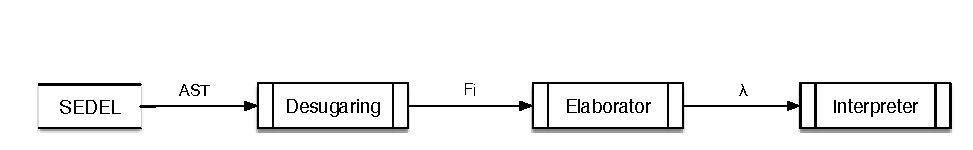
\includegraphics[scale=0.7]{pipeline.eps}
\caption{The pipeline of the implementation.}
  \end{figure}




\end{frame}


\begin{frame}
  \frametitle{Discussion}
  \begin{itemize}
  \item Compared to the original \bname calculus, we have an additional rule,
    which is helpful for the composition of Object Algebras.     \ottusedrule{\ottdruleSubXXR{}}
  \item By this rule, one can derive for example
    $$
    \ottsym{\{} \ottmv{l} \ottsym{:} \mathsf{A} \rightarrow \mathsf{B}
    \ottsym{\}} \,\&\, \ottsym{\{} \ottmv{l} \ottsym{:} \mathsf{C} \rightarrow
    \mathsf{C} \ottsym{\}} <: \ottsym{\{} \ottmv{l} \ottsym{:} \mathsf{A} \,\&\,
    \mathsf{C} \rightarrow \mathsf{B} \,\&\, \mathsf{C} \ottsym{\}}
    $$
  \item Our preliminary meta-theoretic study shows that this rule would not
    endanger the type system.
  \end{itemize}

\end{frame}



\section{Future Work}

\begin{frame}
  \frametitle{Future Work}
  \begin{itemize}
  \item \name is still very simple in term of language features, adding state
    variables, recursive types, etc.
  \item Meta-theory of a relaxed version of \bname: drop disjointness condition in the
    well-formedness of intersection types.
    \begin{itemize}
    \item The relaxed system would allow types such as $\mathsf{Int} \,\&\, \mathsf{Int}$ to exist. Also it would enable the following subtyping rule
      when $A$ and $C$ are not necessarily disjoint:
      \[
        (A \rightarrow B) \,\&\, (C \rightarrow D) <: A \,\&\, C \rightarrow B \,\&\, D
      \]
    \item The introduction rule of merges still require the disjointness
      condition, the values of $\mathsf{Int} \,\&\, \mathsf{Int}$ are those like
      $(3,3)$.
    \item The proof of coherence becomes much challenging, may need contextual
      equivalence and logical relations.
    \end{itemize}



  \end{itemize}
\end{frame}



\end{document}
